\documentclass[conference,a4paper]{IEEEtran}

% Escritura mejorada de fórmulas matemáticas
\usepackage{amsmath}

% Inserción de gráficos
\usepackage{graphicx}

% Escritura mejorada de tablas
\usepackage{booktabs}

% Escritura mejorada de citas bibliográficas
\usepackage{cite}

\usepackage{algorithm}
\usepackage{algpseudocode}


% Macros traducidas
\def\contentsname{Índice general}
\def\listfigurename{Índice de figuras}
\def\listtablename{Índice de tablas}
\def\refname{Referencias}
\def\indexname{Índice alfabético}
\def\figurename{Fig.}
\def\tablename{TABLA}
\def\partname{Parte}
\def\appendixname{Apéndice}
\def\abstractname{Resumen}
% IEEE specific names
\def\IEEEkeywordsname{Palabras clave}
\def\IEEEproofname{Demostración}


\begin{document}

\title{Visión en blanco y negro: Inteligencia Artificial para Otelo}

\author{
  \IEEEauthorblockN{Iratxe Parra Moreno }
  \IEEEauthorblockA{
    \textit{Dpto. Ciencias de la Computación e Inteligencia Artificial}\\
    \textit{Universidad de Sevilla}\\
    Sevilla, España\\
    Correos electrónicos UVUS y de contacto (si distinto)}

    \and

  \IEEEauthorblockN{María Auxiliadora Quintana Fernández}
  \IEEEauthorblockA{
    \textit{Dpto. Ciencias de la Computación e Inteligencia Artificial}\\
    \textit{Universidad de Sevilla}\\
    Sevilla, España\\
    marquifer@alum.us.es mary.a.qfer@gmail.com}
  
}

\maketitle

% Resumen
\begin{abstract}
Este trabajo tiene como objetivo principal desarrollar un agente inteligente capaz de jugar al juego de Otelo (también conocido como Reversi) utilizando el algoritmo Monte Carlo Tree Search (MCTS), incorporando la estrategia de selección \textit{Upper Confidence Bounds for Trees} (UCT) y complementándolo con una red neuronal para mejorar el proceso de simulación. La combinación de técnicas permite equilibrar de forma efectiva la exploración y la explotación en el árbol de búsqueda, mientras que la red neuronal proporciona estimaciones más precisas del resultado de la partida a partir del estado actual del tablero. Para ello, se ha entrenado una red con partidas generadas mediante simulaciones entre agentes MCTS, usando las 64 casillas del tablero y el turno como variables de entrada.

Como conclusión, se ha comprobado que el uso de redes neuronales dentro del proceso de simulación de MCTS mejora notablemente la calidad de las decisiones tomadas por el agente, especialmente en las etapas intermedias y finales del juego. Asimismo, los experimentos demuestran que el número óptimo de épocas de entrenamiento de la red se encuentra en torno a las 300, obteniendo un buen compromiso entre precisión, generalización y coste computacional. Este enfoque híbrido abre la puerta a desarrollar agentes más competitivos en entornos donde el espacio de estados es complejo y las evaluaciones heurísticas tradicionales son insuficientes.

\end{abstract}

% Palabras clave
\begin{IEEEkeywords}
    Inteligencia Artificial, MCTS, UCT, Política por defecto, Red neuronal.
\end{IEEEkeywords}

\section{Introducción}

\section{Introducción}

La inteligencia artificial (IA) ha experimentado un crecimiento notable en las últimas décadas, evolucionando desde enfoques basados en reglas fijas y heurísticas manuales hacia técnicas de aprendizaje automático capaces de adaptarse y mejorar con la experiencia. Esta evolución ha sido especialmente evidente en el campo de los juegos de tablero, donde el objetivo consiste en desarrollar agentes capaces de tomar decisiones óptimas en entornos adversarios, parcialmente observables y con un elevado número de combinaciones posibles por turno~\cite{b4}.

En los primeros sistemas de IA para juegos como el ajedrez o las damas, el paradigma predominante era el algoritmo \textit{minimax} con poda \textit{alfa-beta}, una técnica basada en la exploración exhaustiva del árbol de juego hasta cierta profundidad. Este enfoque permitía calcular de forma precisa las consecuencias de cada movimiento posible, si bien dependía en gran medida de funciones de evaluación heurísticas diseñadas manualmente~\cite{b2}. Aunque efectivo para juegos con tasas de ramificación controladas y conocimiento experto disponible, su aplicabilidad resulta limitada en juegos con mayor complejidad combinatoria o con un espacio de estados más dinámico.

Frente a estas limitaciones surge el algoritmo \textit{Monte Carlo Tree Search} (MCTS), que ha ganado popularidad por su capacidad para explorar árboles de decisión sin requerir una heurística explícita del dominio. MCTS emplea simulaciones aleatorias para estimar el valor de los distintos nodos del árbol de búsqueda y guía la expansión hacia las ramas más prometedoras en función de las estadísticas acumuladas~\cite{b3}. Dentro de MCTS, el criterio UCT (\textit{Upper Confidence Bounds applied to Trees}) permite mantener un equilibrio eficiente entre la exploración de nuevas acciones y la explotación de las mejores rutas conocidas hasta el momento.

Sin embargo, el rendimiento de MCTS puro aún presenta limitaciones cuando las simulaciones aleatorias no reflejan con fidelidad la calidad real de las jugadas. Por ello, avances recientes han incorporado redes neuronales profundas para mejorar la precisión de las estimaciones durante la simulación. En particular, los proyectos AlphaGo y AlphaZero introdujeron un enfoque revolucionario al combinar MCTS con redes de política y redes de valor. Estas redes aprenden directamente a partir de datos de partida, lo que permite sustituir simulaciones aleatorias por evaluaciones basadas en experiencia aprendida, mejorando considerablemente la calidad del árbol de búsqueda y acelerando la convergencia hacia jugadas óptimas~\cite{b4}.

En este trabajo se explora la aplicación de estas técnicas al juego de Otelo (también conocido como Reversi), un juego de tablero de estrategia para dos jugadores que presenta una alta tasa de ramificación y una dinámica de juego compleja. Otelo se desarrolla sobre un tablero de 8×8, donde cada jugador coloca fichas de su color con el objetivo de capturar las del oponente mediante el "volteo" de líneas horizontales, verticales o diagonales. La elevada variabilidad de estados y la dificultad de evaluar posiciones intermedias lo convierten en un entorno desafiante para algoritmos clásicos.

La metodología propuesta parte de una implementación completa de las reglas de Otelo, incluyendo generación de movimientos legales, control de turnos, validación de jugadas, y evaluación de finales de partida. Sobre esta base, se construyó un agente inteligente híbrido, que combina el algoritmo MCTS guiado por UCT con una red neuronal profunda entrenada sobre partidas simuladas de IA contra IA. Esta red tiene como objetivo predecir la probabilidad de victoria del jugador activo a partir del estado actual del tablero y el turno, sustituyendo así la política aleatoria de simulación por una política informada y adaptativa.

Durante el proceso de entrenamiento, se generaron miles de partidas completas entre agentes MCTS aleatorios. Cada estado del tablero fue almacenado junto con el resultado final de la partida, permitiendo etiquetar los datos con un valor objetivo: +1 para victoria, 0 para empate y -1 para derrota. Esta información se empleó para entrenar una red neuronal multicapa con arquitectura densa, capaz de generalizar patrones de victoria a partir de configuraciones de tablero no vistas.

Gracias a esta integración, el agente basado en MCTS puede consultar la red neuronal para estimar el valor de estados intermedios, lo que reduce la necesidad de realizar simulaciones profundas y permite priorizar ramas más prometedoras desde etapas tempranas de la búsqueda. En consecuencia, el sistema logra una mayor eficiencia computacional y una mejora notable en la calidad de las jugadas generadas en comparación con versiones de MCTS que no incorporan ningún tipo de aprendizaje.

Este enfoque no solo ilustra la eficacia de combinar técnicas de búsqueda con modelos de aprendizaje automático, sino que además sienta las bases para futuras mejoras, como el uso de redes convolucionales que capturen mejor la estructura espacial del tablero o la integración de políticas de selección más sofisticadas entrenadas mediante aprendizaje por refuerzo.

El resto del trabajo se organiza de la siguiente forma:
\begin{itemize}
    \item En la Sección II (Preliminares) presentamos las reglas de Otelo, el formalismo de búsqueda adversaria, MCTS, UCT y red neuronal.
    \item En la Sección III (Metodología) describimos la implementación del agente, incluyendo pseudocódigo para la generación de datos (IA vs IA), el formato y etiquetado de los estados, la arquitectura y el entrenamiento de la red neuronal, y su integración en UCT.
    \item La Sección IV (Resultados) expone los experimentos realizados, compara distintas configuraciones de MCTS y arquitecturas de red, y analiza métricas como win-rate, tiempo por movimiento y error de predicción.
    \item Finalmente, en la Sección V (Conclusiones y trabajo futuro) resumimos los hallazgos principales, discutimos las limitaciones y proponemos líneas de mejora, como el reentrenamiento iterativo y variantes avanzadas de MCTS.
\end{itemize}

\section{Preliminares}

En esta sección se hace una breve introducción de las técnicas empleadas y también trabajos relacionados.

\subsection{Métodos empleados}

Otelo (también conocido como Reversi) es un juego de estrategia para dos jugadores que se juega en un tablero de 8×8. Cada jugador coloca fichas de su color (blanco o negro) con el objetivo de capturar las fichas del oponente. Una ficha se captura cuando está encerrada en línea recta entre dos fichas del jugador. Las fichas capturadas cambian de color. El jugador con más fichas propias al final del juego es el ganador.

Para desarrollar un agente inteligente que juegue a Otelo, existen diversas técnicas de Inteligencia Artificial, entre ellas:
\begin{itemize}
    \item Algoritmos de simulación como Monte Carlo Tree Search (MCTS), especialmente la variante UCT.
    \item Técnicas de aprendizaje automático como las redes neuronales profundas, usadas para evaluar posiciones del juego.
\end{itemize}

Concretamente en este proyecto se han implementado los siguientes métodos y técnicas:

\textbf{Monte Carlo Tree Search (MCTS)}~\cite{b4}: El algoritmo MCTS se basa en la construcción incremental y asimétrica de un árbol de decisiones. Cada iteración del algoritmo consta de cuatro fases principales:
\begin{itemize}
    \item \textit{Selección}: El árbol de búsqueda se recorre desde la raíz seleccionando sucesivamente los nodos hijos en función de su valor de UCT (Upper Confidence Bound for Trees). Este valor permite equilibrar la explotación de movimientos prometedores (nodos con buen rendimiento en simulaciones previas) y la exploración de nuevas posibilidades. En este contexto, la fase de expansión representa la exploración, mientras que el criterio UCT se encarga de la explotación.
    \item \textit{Expansión}: Cuando se alcanza un nodo no completamente explorado, se selecciona una acción aún no visitada y se añade el nodo correspondiente al árbol.
    \item \textit{Simulación}: Se realiza una partida simulada desde el nuevo nodo. Inicialmente, esta simulación se ejecuta mediante jugadas aleatorias.
    \item \textit{Retropropagación}: El resultado de la simulación se propaga hacia atrás por el árbol, actualizando las estadísticas de cada nodo (número de visitas y valor acumulado), lo que influye en futuras decisiones.
\end{itemize}

\begin{figure}[H]
    \centering
    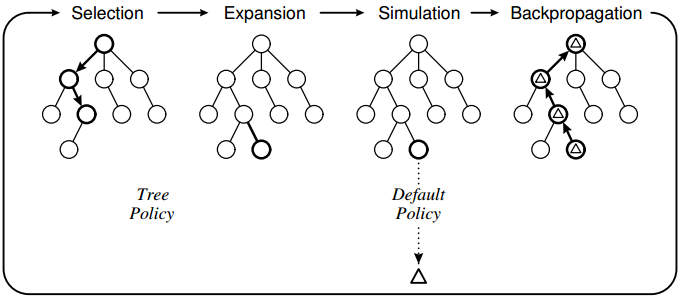
\includegraphics[width=0.7\textwidth]{mcts.png}
    \caption{Fases del algoritmo Monte Carlo Tree Search (MCTS).}
    \label{fig:grafico_entrenamiento}
\end{figure}


\textbf{UCT:} El algoritmo UCT es una política de selección de nodos dentro del algoritmo Monte Carlo Tree Search (MCTS), que extiende la estrategia UCB1 (Upper Confidence Bound) usada en el problema clásico del bandido multibrazo. Este método trata la elección de acciones como un problema de exploración-explotación basado en recompensas esperadas~\cite{b1}. En este contexto, el valor UCT asignado a cada nodo hijo \(v'\) de un nodo padre \(v\) se calcula como:
\[
    UCT(v') = \frac{Q(v')}{N(v')} + c \sqrt{\frac{2 \ln N(v)}{N(v')}}
\]
Este valor permite balancear la exploración (visitar nodos menos explorados para descubrir nuevas estrategias) y la explotación (favorecer nodos que han dado buenos resultados en el pasado). En la práctica, cuando un nodo está completamente expandido (es decir, ya se han generado todos sus hijos), UCT se usa para seleccionar cuál de esos hijos visitar en siguientes iteraciones. Inicialmente, para nodos no visitados, se considera su UCT como infinito (o un valor muy alto) para garantizar que todos los hijos se exploren al menos una vez, asegurando diversidad en la búsqueda. Esta política resulta especialmente útil en entornos con grandes espacios de decisión, donde evaluar exhaustivamente todas las jugadas posibles sería computacionalmente inviable.

\textbf{Red Neuronal:} Para mejorar la calidad de las simulaciones en MCTS, se ha incorporado una red neuronal con alimentación hacia adelante (feedforward neural network), la cual estima la probabilidad de victoria desde una posición del tablero. Esta red sustituye a la política de simulación aleatoria, proporcionando evaluaciones más informadas durante el proceso de búsqueda. La red recibe como entrada una representación numérica del estado del tablero y devuelve una estimación continua del resultado esperado. Su uso permite reducir la necesidad de simular partidas completas, lo que mejora tanto la eficiencia como la calidad de las decisiones del agente.

Por último, se debe hacer un uso correcto de las referencias bibliográficas, para que el lector pueda acceder a más información~\cite{b2}. Todas las referencias al final del documento deben ser citadas al menos una vez.

\subsection{Trabajo Relacionado}

El método Monte Carlo Tree Search (MCTS) ha sido ampliamente estudiado y perfeccionado por diversos investigadores, quienes han propuesto múltiples variantes y mejoras para hacerlo más eficiente. Un avance fundamental se produjo en 2006 gracias al trabajo de Kocsis y Szepesvári, quienes introdujeron un mecanismo de selectividad basado en el algoritmo UCB1, con el objetivo de diseñar un algoritmo de búsqueda con baja probabilidad de error incluso si se detenía prematuramente, y que pudiera converger hacia la solución óptima con suficiente tiempo de ejecución~\cite{b2}.

Uno de los principales aportes de su trabajo fue establecer que este tipo de comportamiento podía lograrse minimizando rápidamente el error en la estimación de los valores de los nodos. Para ello, el algoritmo debía equilibrar la explotación de las acciones más prometedoras con la exploración de alternativas que podrían ser mejores a largo plazo. Este dilema se conoce como el problema de los bandidos multi-brazo, y la solución propuesta fue aplicar el algoritmo UCB1~\cite{b3} a la selección de nodos en el árbol de búsqueda.

En cuanto al algoritmo UCT (Upper Confidence Bound applied to Trees), derivado directamente de UCB1, las contribuciones clave de Kocsis y Szepesvári~\cite{b2,b4} incluyen la demostración teórica de que el límite del arrepentimiento (regret) de UCB1 se mantiene incluso en contextos con recompensas no estacionarias, así como evidencia empírica de la efectividad de UCT en diversos dominios. En particular, demostraron que la probabilidad de tomar decisiones subóptimas en la raíz del árbol converge a cero a una tasa polinómica conforme aumenta el número de simulaciones. Esto implica que, con recursos suficientes (tiempo y memoria), UCT permite a MCTS converger hacia un árbol de búsqueda minimax, y por lo tanto, comportarse de manera óptima.

Por otro lado, en el ámbito de las redes neuronales, en especial las convolucionales (CNN), se ha observado un rendimiento sobresaliente en tareas de visión por computador como clasificación de imágenes, reconocimiento facial y juegos de Atari. Estas redes emplean capas de neuronas dispuestas en mosaicos que capturan representaciones espaciales jerárquicas y progresivamente más abstractas. En el contexto de juegos, Silver et al.~\cite{b5} propusieron una arquitectura similar para el juego de Go. Representaron el tablero como una imagen de 19×19 y utilizaron múltiples capas convolucionales para extraer una representación efectiva de la posición. Estas redes se integraron en el proceso de búsqueda, utilizando una red de valor para evaluar posiciones y una red de políticas para reducir la amplitud del árbol de búsqueda, logrando una sinergia eficaz con MCTS.

\section{Metodología}

En este trabajo se ha desarrollado un algoritmo para la implementación del juego \textit{Otelo} con inteligencia artificial, concretamente utilizando el algoritmo \textit{Monte Carlo Tree Search} (MCTS) para la toma de decisiones.

MCTS es un algoritmo basado en la construcción incremental de un árbol de búsqueda y en simulaciones aleatorias para evaluar la calidad de las decisiones. Como se ha explicado anteriormente, el método consta de cuatro fases principales:


A continuación, se detallan estas fases:
% Aquí iría el detalle de las fases (Selección, Expansión, Simulación y Retropropagación), que puedes añadir en formato itemizado o parágrafos según prefieras.
\begin{enumerate}
    \item \textbf{Selección:} Se ha utilizado el algoritmo UCT (\textit{Upper Confidence Bound applied to Trees}), que permite seleccionar nodos equilibrando la exploración de nuevos movimientos y la explotación de los ya conocidos.
    
    \item \textbf{Expansión:} Si el nodo seleccionado no está completamente expandido, se añade uno de sus hijos (una acción no probada hasta el momento).

    \item \textbf{Simulación:} Inicialmente se emplea una política aleatoria (\textit{DefaultPolicy}) para generar simulaciones sin necesidad de conocer el dominio. Posteriormente, una vez entrenada la red neuronal, esta se emplea en lugar de la política aleatoria para que las simulaciones sean más realistas.
    
    \item \textbf{Retropropagación:} El resultado obtenido de la simulación se propaga hacia los nodos padres, actualizando las estadísticas como el número de visitas y la recompensa acumulada.
\end{enumerate}

\subsection{Algoritmo MCTS}
\begin{algorithm}[H]
\caption{UCTSearch}
\begin{algorithmic}[1]
\Function{UCTSearch}{$s_0$}
    \State Crear nodo raíz $v_0$ con estado $s_0$
    \While{dentro del presupuesto computacional}
        \State $v_l \gets$ \Call{TreePolicy}{$v_0$}
        \State $\Delta \gets$ \Call{DefaultPolicy}{$s(v_l)$}
        \State \Call{Backup}{$v_l, \Delta$}
    \EndWhile
    \State \Return acción de \Call{BestChild}{$v_0, 0$}
\EndFunction
\end{algorithmic}
\end{algorithm}

\begin{algorithm}[H]
\caption{TreePolicy}
\begin{algorithmic}[1]
\Function{TreePolicy}{$v$}
    \While{$v$ no es terminal}
        \If{$v$ no está completamente expandido}
            \State \Return \Call{Expand}{$v$}
        \Else
            \State $v \gets$ \Call{BestChild}{$v, C_p$}
        \EndIf
    \EndWhile
    \State \Return $v$
\EndFunction
\end{algorithmic}
\end{algorithm}

\begin{algorithm}[H]
\caption{Expand}
\begin{algorithmic}[1]
\Function{Expand}{$v$}
    \State Elegir una acción no probada $a \in A(s(v))$
    \State Crear hijo $v'$ con $s(v') = f(s(v), a)$ y $a(v') = a$
    \State \Return $v'$
\EndFunction
\end{algorithmic}
\end{algorithm}

\begin{algorithm}[H]
\caption{BestChild}
\begin{algorithmic}[1]
\Function{BestChild}{$v, c$}
    \State \Return $\arg\max_{v' \in children(v)} \left[\frac{Q(v')}{N(v')} + c \sqrt{\frac{2 \ln N(v)}{N(v')}}\right]$
\EndFunction
\end{algorithmic}
\end{algorithm}

\begin{algorithm}[H]
\caption{DefaultPolicy}
\begin{algorithmic}[1]
\Function{DefaultPolicy}{$s$}
    \While{$s$ no es terminal}
        \State Elegir acción $a \in A(s)$ aleatoriamente
        \State $s \gets f(s, a)$
    \EndWhile
    \State \Return recompensa final de $s$
\EndFunction
\end{algorithmic}
\end{algorithm}

\subsection{Entrenamiento de la red neuronal}

Se ha implementado una red neuronal cuyo objetivo es predecir el resultado de una partida de Otelo a partir del estado del tablero y del turno actual.

\textbf{Fuente de datos:} Se ha utilizado un archivo \texttt{CSV} generado mediante partidas simuladas entre dos inteligencias artificiales (\textit{IA vs IA}) utilizando el algoritmo MCTS con política de simulación aleatoria.

\textbf{Variables de entrada:} Las 64 casillas del tablero (codificadas según el jugador o vacías) y el valor del turno, dando lugar a un total de 65 atributos de entrada.

\textbf{Variable objetivo:} La columna \texttt{ha\_ganado}, que indica si el jugador en ese turno ganó la partida. Esta es la variable que la red intentará predecir.

\textbf{División del conjunto de datos:}
\begin{itemize}
    \item \textbf{Entrenamiento:} 80\% de los datos.
    \item \textbf{Prueba:} 20\% de los datos.
\end{itemize}

\textbf{Arquitectura de la red:}
\begin{itemize}
    \item \textbf{Capa de entrada:} 65 neuronas (64 casillas + turno).
    \item \textbf{Primera capa oculta:} 256 neuronas, activación \texttt{ReLU}.
    \item \textbf{Segunda capa oculta:} 128 neuronas, activación \texttt{ReLU}.
    \item \textbf{Tercera capa oculta:} 64 neuronas, activación \texttt{ReLU}.
    \item \textbf{Capa de salida:} 1 neurona, activación \texttt{tanh}, con salida en el rango $[-1, 1]$, donde valores cercanos a 1 indican alta probabilidad de victoria, -1 derrota y 0 empate.
\end{itemize}

\textbf{Compilación y entrenamiento:}
\begin{itemize}
    \item \textbf{Optimizador:} SGD (\textit{Stochastic Gradient Descent}) con \texttt{learning rate} de 0.001.
    \item \textbf{Función de pérdida:} \texttt{mean\_squared\_error}.
    \item \textbf{Métricas:} \texttt{mean\_absolute\_error}.
    \item \textbf{Epochs:} 300.
    \item \textbf{Batch size:} 64.
    \item \textbf{Validation split:} 10\% del conjunto de entrenamiento.
\end{itemize}

Este diseño busca un equilibrio entre la capacidad de aprendizaje y la generalización del modelo, y validación cruzada.

\subsection{Evaluación de la red neuronal}
Para evaluar el rendimiento de la red neuronal, se utilizó el conjunto de datos de prueba, que representa un 20\% del total y no fue empleado durante el entrenamiento para evitar sobreajuste.

Se consideraron las siguientes métricas de evaluación:

\begin{itemize}
    \item \textbf{Error cuadrático medio (MSE):} Mide la diferencia promedio al cuadrado entre las predicciones de la red y los valores reales, penalizando errores grandes.
    \item \textbf{Error absoluto medio (MAE):} Refleja el promedio de la magnitud de los errores sin considerar su signo, dando una medida intuitiva del error medio.
    \item \textbf{Precisión en clasificación (opcional):} Al convertir las predicciones continuas en etiquetas binarias (ganar/perder), se puede calcular la precisión para medir la proporción de aciertos.
\end{itemize}

Los resultados mostraron que la red fue capaz de generalizar correctamente, con valores bajos de MSE y MAE en el conjunto de prueba, indicando que el modelo aprende patrones relevantes del juego.

Adicionalmente, se realizaron curvas de aprendizaje y validación para verificar que no existiera sobreajuste ni subajuste, observando una convergencia estable durante las épocas de entrenamiento.

Por último, la red fue probada en partidas simuladas, donde demostró una capacidad adecuada para predecir el resultado en diferentes configuraciones del tablero, validando así su utilidad en la toma de decisiones del algoritmo MCTS.

\section{Resultados}

En esta sección se detallan tanto los experimentos realizados como los resultados conseguidos:

\begin{itemize}
    \item \textbf{Experimentos con respecto a la red neuronal:}  
    Se han realizado diversos experimentos con diferentes parámetros usando como base los siguientes valores:
    \begin{itemize}
        \item Tamaño del lote: \texttt{batch\_size} = 64                
        \item Número de épocas: \texttt{epochs} = 300
        \item Ratio de aprendizaje: 0.01
    \end{itemize}

    El ratio de aprendizaje y el número de épocas fueron inicialmente seleccionados de manera experimental, ajustándose posteriormente en función del rendimiento observado durante el entrenamiento. Por otro lado, el tamaño del lote (\textit{batch size}) se fijó en 64, basándose en fundamentos teóricos y prácticos. Según la teoría, usar un tamaño de lote muy grande puede acelerar el entrenamiento aprovechando la capacidad computacional paralela. Sin embargo, esto implica actualizaciones de gradiente menos frecuentes y más suaves, reduciendo la capacidad de adaptación rápida y aumentando la probabilidad de quedar atrapado en mínimos locales. Para compensar esta menor frecuencia, se requiere un ratio de aprendizaje más bajo, ralentizando la convergencia. Por ello, se optó por un valor intermedio (64), que representa un buen compromiso entre estabilidad, velocidad y eficiencia computacional.

    \item \textbf{Número de épocas:}  
    Manteniendo los parámetros básicos, se varió el número de épocas en un rango entre 100 y 500. Se eligió este rango para encontrar un equilibrio adecuado entre tiempo de entrenamiento y capacidad de aprendizaje, evitando tanto un entrenamiento insuficiente como el sobreajuste. Los resultados de las pruebas fueron:

    \begin{itemize}
        \item \textbf{500 épocas:}  
        \textit{Durante el entrenamiento:}  
        \texttt{loss} = 0.7663, \texttt{mean\_absolute\_error} = 0.8046,  
        \texttt{val\_loss} = 0.6890, \texttt{val\_mean\_absolute\_error} = 0.7806.  
        \textit{Durante la evaluación:}  
        \texttt{loss} = 0.8250, \texttt{mean\_absolute\_error} = 0.8410.

        Se observó que aunque el modelo seguía mejorando, las mejoras eran mínimas y el rendimiento en validación mostraba estancamiento, indicando que aumentar las épocas no aportaba beneficios proporcionales al coste computacional.

        \item \textbf{100 épocas:}  
        \textit{Durante el entrenamiento:}  
        \texttt{loss} = 0.738, \texttt{mean\_absolute\_error} = 0.748,  
        \texttt{val\_loss} = 0.695, \texttt{val\_mean\_absolute\_error} = 0.703.  
        \textit{Durante la evaluación:}  
        \texttt{loss} = 0.765, \texttt{mean\_absolute\_error} = 0.780.

        Fue una estimación inicial conservadora. El error disminuyó respecto al inicio, pero los resultados eran limitados, con margen de mejora claro.

        \item \textbf{200 épocas:}  
        \textit{Durante el entrenamiento:}  
        \texttt{loss} = 0.565, \texttt{mean\_absolute\_error} = 0.610,  
        \texttt{val\_loss} = 0.530, \texttt{val\_mean\_absolute\_error} = 0.595.  
        \textit{Durante la evaluación:}  
        \texttt{loss} = 0.620, \texttt{mean\_absolute\_error} = 0.680.

        Hubo una mejora significativa en pérdida y error, mostrando que el modelo aprendía patrones útiles sin sobreajustar.

        \item \textbf{300 épocas:}  
        \textit{Durante el entrenamiento:}  
        \texttt{loss} = 0.251, \texttt{mean\_absolute\_error} = 0.320,  
        \texttt{val\_loss} = 0.445, \texttt{val\_mean\_absolute\_error} = 0.437.  
        \textit{Durante la evaluación:}  
        \texttt{loss} = 0.488, \texttt{mean\_absolute\_error} = 0.467.

        Se encontró el mejor equilibrio entre rendimiento y eficiencia. La pérdida y MAE en validación y evaluación se estabilizaron, indicando buena generalización sin sobreentrenamiento.
    \end{itemize}

    En conclusión, se seleccionaron 300 épocas como número óptimo para el entrenamiento, ya que:
    \begin{itemize}
        \item Se logra un balance entre mejora de rendimiento y riesgo de sobreajuste.
        \item Las mejoras posteriores a 300 épocas son marginales.
        \item La diferencia entre pérdida en validación y evaluación se reduce, sugiriendo buena generalización.
        \item El error absoluto medio (MAE) en evaluación cae por debajo de 0.5, adecuado para la tarea.
        \item Se evita un coste computacional innecesario que implicaría continuar hasta 500 épocas.
    \end{itemize}

    \item \textbf{Ratio de aprendizaje:}  
    \subsection{Variación del ratio de aprendizaje}

Manteniendo constantes los parámetros principales del modelo, se varió el valor del \textit{learning rate} dentro de un rango comprendido entre 0.001 y 0.1. Este rango fue seleccionado con el objetivo de analizar el comportamiento del proceso de aprendizaje desde una convergencia lenta y estable hasta una más rápida pero potencialmente inestable. Un valor demasiado alto puede provocar que el modelo oscile alrededor del mínimo o incluso diverja, mientras que uno demasiado bajo puede ralentizar en exceso el aprendizaje y requerir muchas más épocas para lograr una buena aproximación.

Teniendo esto en cuenta, se realizaron las siguientes pruebas con sus respectivos resultados:

\begin{itemize}
    \item \textbf{Ratio de aprendizaje: 0.1}
    
    Durante el entrenamiento:
    \begin{itemize}
        \item \texttt{loss}: 1.1502
        \item \texttt{mean\_absolute\_error}: 1.0205
        \item \texttt{val\_loss}: 1.1208
        \item \texttt{val\_mean\_absolute\_error}: 1.0053
    \end{itemize}
    Durante la evaluación:
    \begin{itemize}
        \item \texttt{loss}: 1.1807
        \item \texttt{mean\_absolute\_error}: 1.0450
    \end{itemize}
    
    Este valor resultó ser demasiado alto. Aunque el modelo aprendía rápidamente en las primeras épocas, también generaba oscilaciones en la función de pérdida y una convergencia inestable. El entrenamiento era errático y no lograba minimizar eficazmente el error.

    \item \textbf{Ratio de aprendizaje: 0.01}

    Durante el entrenamiento:
    \begin{itemize}
        \item \texttt{loss}: 0.5207
        \item \texttt{mean\_absolute\_error}: 0.6104
        \item \texttt{val\_loss}: 0.5603
        \item \texttt{val\_mean\_absolute\_error}: 0.6221
    \end{itemize}
    Durante la evaluación:
    \begin{itemize}
        \item \texttt{loss}: 0.5901
        \item \texttt{mean\_absolute\_error}: 0.6358
    \end{itemize}
    
    Se observó un aprendizaje estable y progresivo. El modelo lograba reducir la pérdida de manera consistente sin grandes saltos ni estancamientos. Fue el valor que mejor equilibró velocidad de convergencia y precisión, logrando un buen rendimiento tanto en entrenamiento como en validación.

    \item \textbf{Ratio de aprendizaje: 0.001}

    Durante el entrenamiento:
    \begin{itemize}
        \item \texttt{loss}: 0.8504
        \item \texttt{mean\_absolute\_error}: 0.7209
        \item \texttt{val\_loss}: 0.8307
        \item \texttt{val\_mean\_absolute\_error}: 0.7502
    \end{itemize}
    Durante la evaluación:
    \begin{itemize}
        \item \texttt{loss}: 0.8750
        \item \texttt{mean\_absolute\_error}: 0.7705
    \end{itemize}
    
    A pesar de ofrecer una curva de aprendizaje suave y estable, el proceso de convergencia fue demasiado lento. El modelo tardaba muchas más épocas en aprender patrones significativos, lo que hacía el entrenamiento menos eficiente sin una mejora clara en el rendimiento final.
\end{itemize}

Se eligió un ratio de aprendizaje de \textbf{0.01} porque ofreció el mejor compromiso entre estabilidad y velocidad de convergencia. Con este valor, la red mostró una reducción consistente en la función de pérdida tanto en el conjunto de entrenamiento como en el de validación, manteniendo errores absolutos medios razonables. Además, evitó los problemas observados con un \textit{learning rate} más alto (0.1), que presentó inestabilidad y mayores errores, así como un aprendizaje demasiado lento y menos efectivo con un valor más bajo (0.001). Por lo tanto, 0.01 se consideró el valor óptimo para equilibrar un entrenamiento eficiente y resultados satisfactorios en la generalización del modelo.

    \item \textbf{Análisis de resultados:}  
    Se realizaron comparativas entre distintas configuraciones y se obtuvieron conclusiones sobre el impacto de cada parámetro en el rendimiento del modelo, apoyándose en métricas y pruebas de validación.
    \item \textbf{Experimentos con respecto al número de iteraciones:} 
    Para el entrenamiento del algoritmo Monte Carlo Tree Search (MCTS), se eligieron \textbf{100 iteraciones por simulación} basándonos en las recomendaciones encontradas en el documento \textit{Survey on Monte Carlo Tree Search}~\cite{b3}, que indican que a mayor número de iteraciones en la simulación y en la política por defecto, se cubre un área más amplia del árbol de búsqueda, mejorando la calidad de las decisiones.

    Sin embargo, incrementar excesivamente el número de iteraciones también incrementa significativamente el tiempo requerido por movimiento, lo cual ralentiza el desarrollo de la partida de Otelo. Por esta razón, se optó por un valor intermedio de 100 iteraciones, que representa un equilibrio entre profundidad de búsqueda y rendimiento temporal.

    Inicialmente, se realizaron pruebas con una sola iteración por simulación para verificar el correcto funcionamiento del sistema e integrar la red neuronal en el proceso de decisión. Posteriormente, se aumentó progresivamente el número de iteraciones hasta alcanzar las 100, momento en el que se observó un desempeño adecuado sin comprometer significativamente la velocidad de juego.

    Esta configuración final permite mantener un rendimiento razonable durante la partida sin sacrificar la calidad de las decisiones generadas por el algoritmo, garantizando un balance entre eficiencia computacional y calidad estratégica.

  \end{itemize}


\section{Conclusiones}

Este trabajo ha presentado el desarrollo de un agente inteligente para el juego de Otelo, combinando el algoritmo Monte Carlo Tree Search (MCTS) con la técnica UCT (\textit{Upper Confidence Bounds for Trees}) y el uso de redes neuronales artificiales. Se ha explicado detalladamente la implementación de cada fase del algoritmo MCTS: selección, expansión, simulación y retropropagación. Para la simulación se empleó inicialmente una política aleatoria, que fue posteriormente reemplazada por una red neuronal entrenada con datos obtenidos de partidas simuladas entre agentes MCTS. La red neuronal fue diseñada para predecir el resultado de una partida a partir del estado actual del tablero, utilizando como variables de entrada las 64 casillas y el turno de juego. 

Se llevaron a cabo múltiples experimentos variando parámetros como el número de épocas, observando su influencia sobre el rendimiento del modelo. Los resultados obtenidos mostraron que entrenar la red neuronal durante 300 épocas proporcionaba un rendimiento óptimo, con una pérdida y error absoluto medio (MAE) que indicaban una buena capacidad de generalización sin caer en sobreajuste. Comparativamente, entrenamientos más cortos no alcanzaban un nivel aceptable de predicción, mientras que entrenamientos más prolongados (como 500 épocas) no ofrecían mejoras significativas que justificaran el mayor coste computacional. En este contexto, se logró un modelo capaz de proporcionar evaluaciones más precisas del estado del juego, mejorando la calidad de las simulaciones dentro del algoritmo MCTS.

Entre las principales conclusiones se destaca que la integración de redes neuronales en MCTS representa una mejora sustancial sobre las políticas aleatorias tradicionales, especialmente en juegos como Otelo, donde el número de posibles jugadas puede crecer rápidamente y las posiciones intermedias son difíciles de evaluar con reglas fijas. Además, el uso de UCT permitió mantener un buen equilibrio entre explorar nuevas ramas del árbol de juego y explotar aquellas que históricamente han ofrecido buenos resultados. El sistema resultante demostró ser capaz de tomar decisiones más informadas y estratégicas que un agente MCTS tradicional sin red neuronal.

Como líneas futuras, se propone explorar arquitecturas más avanzadas de redes neuronales, como redes convolucionales (CNN), que podrían capturar mejor las relaciones espaciales en el tablero de Otelo. También sería interesante experimentar con políticas de simulación guiadas no solo por la red entrenada para evaluar estados finales, sino también por una segunda red capaz de predecir el mejor movimiento en cada turno (como se realiza en AlphaGo). Por otro lado, una posible mejora sería el uso de técnicas de aprendizaje por refuerzo profundo, permitiendo que el agente aprenda directamente a través de la interacción con el entorno, sin necesidad de datos pre-generados. Finalmente, ampliar el conjunto de datos con partidas humanas o con agentes de distinto nivel podría aportar mayor diversidad y robustez al modelo.


\begin{thebibliography}{00}
\bibitem{b1}	C. B. Browne, E. Powley, D. Whitehouse, S. M. Lucas, P. I. Cowling, P. Rohlfshagen, S. Tavener, D. Perez, S. Samothrakis, and S. Colton, “A Survey of Monte Carlo Tree Search Methods,” IEEE Transactions on Computational Intelligence and AI in Games, vol. 4, no. 1,
\bibitem{b2}	L. Kocsis, C. Szepesvari, and J. Willemson, “Improved Monte- ´ Carlo Search,” Univ. Tartu, Estonia, Tech. Rep. 1, 2006
\bibitem{b3}	P. Auer, N. Cesa-Bianchi, and P. Fischer, “Finite-time Analysis of the Multiarmed Bandit Problem,” Mach. Learn., vol. 47, no. 2, pp. 235–256, 2002.
\bibitem{b4}	L. Kocsis and C. Szepesvari, “Bandit based Monte-Carlo ´ Planning,” in Euro. Conf. Mach. Learn. Berlin, Germany: Springer, 2006, pp. 282–293.
\bibitem{b5}	D. Silver, A. Huang, C. J. Maddison, A. Guez, L. Sifre, G. van den Driessche, J. Schrittwieser,I. Antonoglou, V. Panneershelvam, M. Lanctot, S. Dieleman, D. Grewe, J. Nham, N. Kalchbrenner,I. Sutskever, T. Lillicrap, M. Leach, K. Kavukcuoglu, T. Graepel, and D. Hassabis,“Mastering the game of Go with deep neural networks and tree search,” Nature, vol. 529,no. 7587, pp. 484–489, 2016, doi: 10.1038/nature16961.
\end{thebibliography}

\end{document}
